\chapter{Results}\label{chap:results}
\begin{overview}
  Results of the techniques whose implementation was discussed in the previous part are shown here.  
  The result of various event identification techniques are shown, followed by examples of models built using the Modelica package and the results of the simulation of these models.
\end{overview}

\section{Segmentation}\label{sec:res:segmentation}
%TODO: This was ripped from the ESCAPE-21 article.
Figure~\ref{fig:segmentationresults} shows some of the results the automated segmentation the sample input data.  
Note that this is a subset of all the fits done, for illustrative purposes.  

\begin{figure}[htbp]
  \centering
  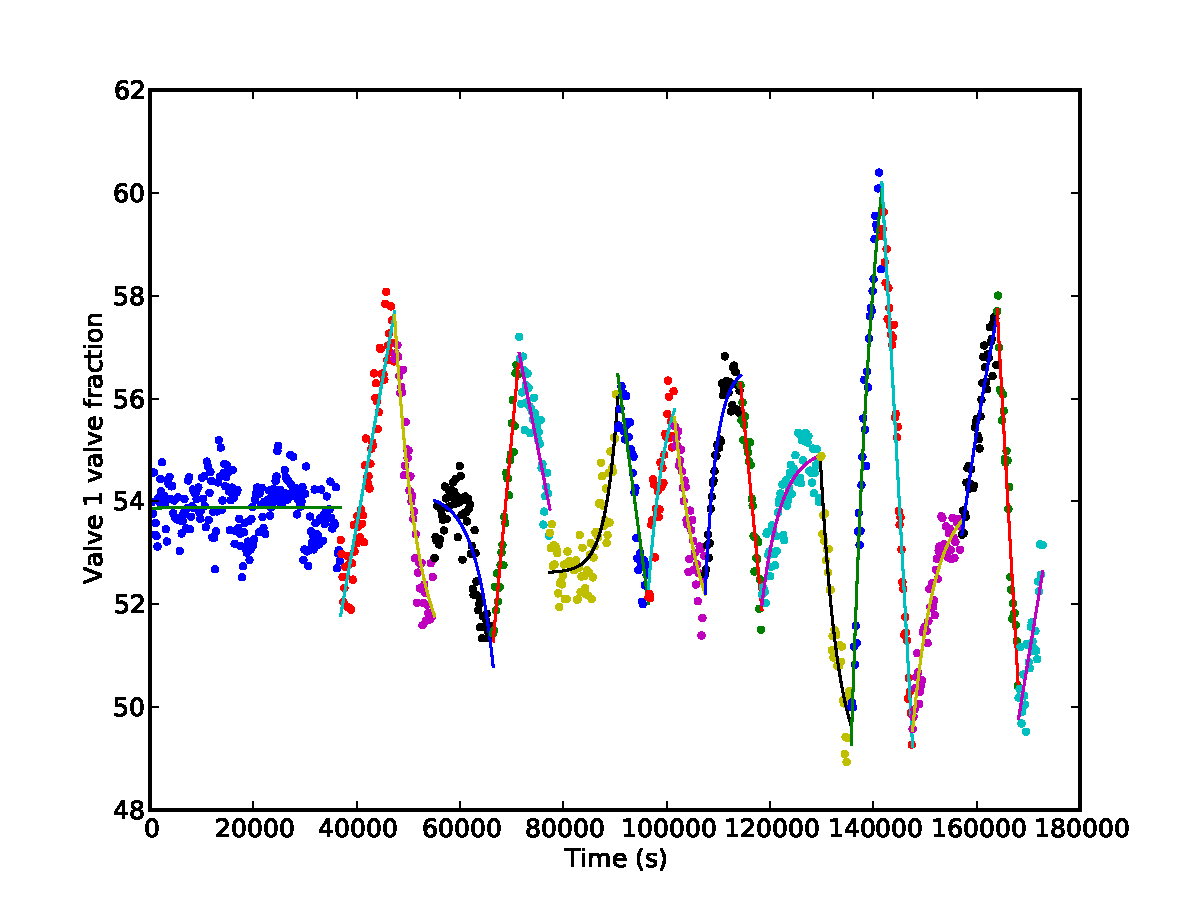
\includegraphics[width=0.7\textwidth]{segmentedsignal}
  
(a)

  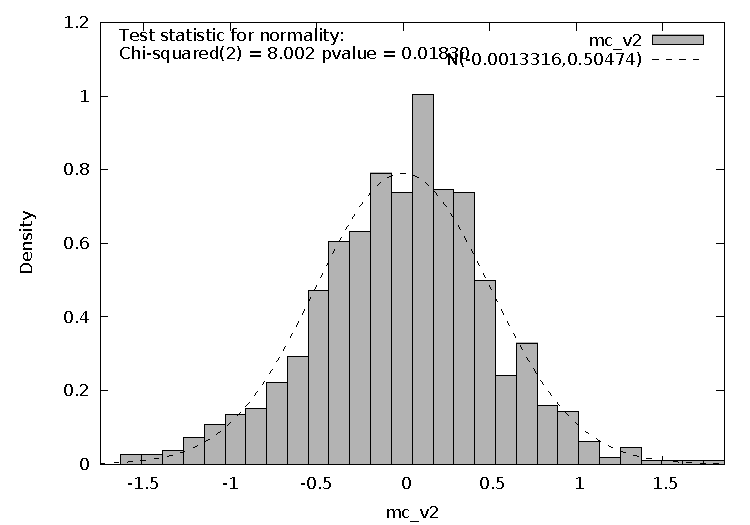
\includegraphics[width=0.44\textwidth]{teresidualnormality}

(b)

  \caption{Segmentation and signal generation results for TE valve input signal.  The residuals are normally distributed.}
  \label{fig:segmentationresults}
\end{figure}

The transitions were analysed for all the fits obtained.

The overall residuals were determined to have be approximately
normally distributed with a standard deviation near 0.5 as shown in Figure~\ref{fig:segmentationresults}.  
This increases the confidence in the segmentation as TE code makes use of normally distributed noise signals.

\subsection{Top-down}

\subsection{Bottom-up}

\subsection{Test signals}
To illustrate the type of result that is obtained using the technique, we show the results on a a signal consisting of 6 events, attempting to fit 4 events.  
Figure~\ref{fig:front_evolution} shows the evolution of the Pareto front in terms of fit complexity and RMS error for different numbers of iterations.

\begin{figure}[htbp]
  \centering
  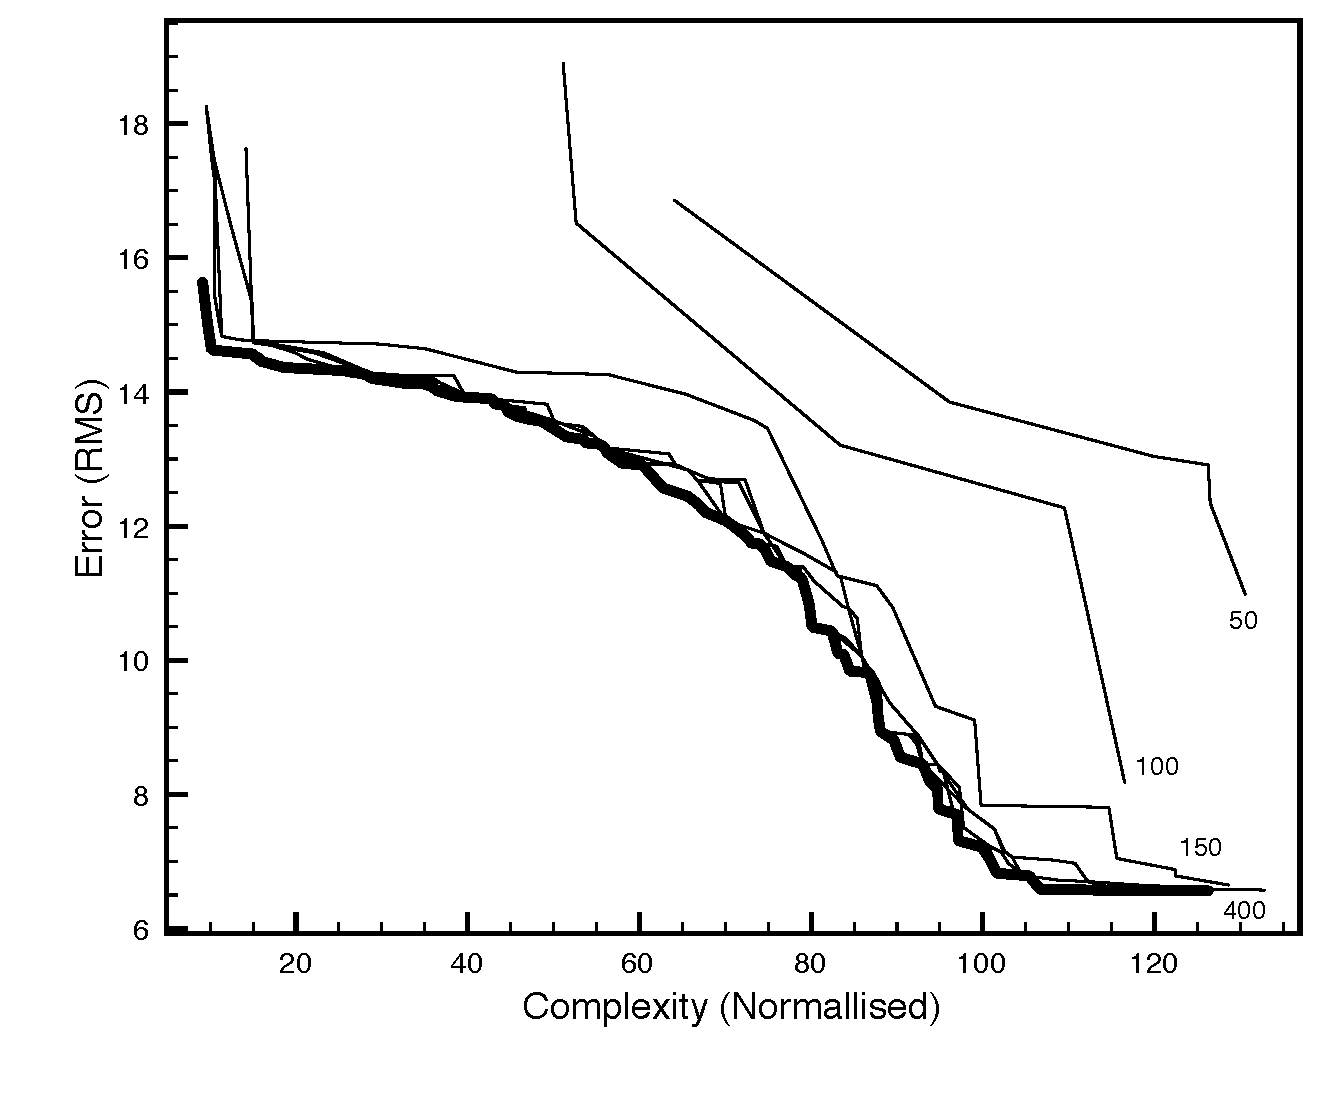
\includegraphics[width=0.7\textwidth]{front_evolution}
  \caption{Evolution of Pareto Front for 6 events being fit by 4 events.}
  \label{fig:front_evolution}
\end{figure}

It should be noted that, although the front seems to be converging, population based multi-objective optimisation algorithms can not guarantee convergence with a finite archive.  
This is due to the pruning that must inevitably be done when the archive is full.
Figure~\ref{fig:front_evolution} does, however, show that the front has not receded.

\subsection{Real-life signals}


\section{Models}

\section{Distillation column model}
\subsection{Simulation accuracy}
To verify the accuracy of the model, it was run simultaneously with the column.  
Figure~\ref{fig:comparison} shows the results of a sample run during which the feed flow rate was varied.  
The distillate drum level and the top plate (plate 1) temperature are shown to illustrate the behaviour of the column and the model.

\label{sec:results}
\begin{figure}[htbp]
  \centering
  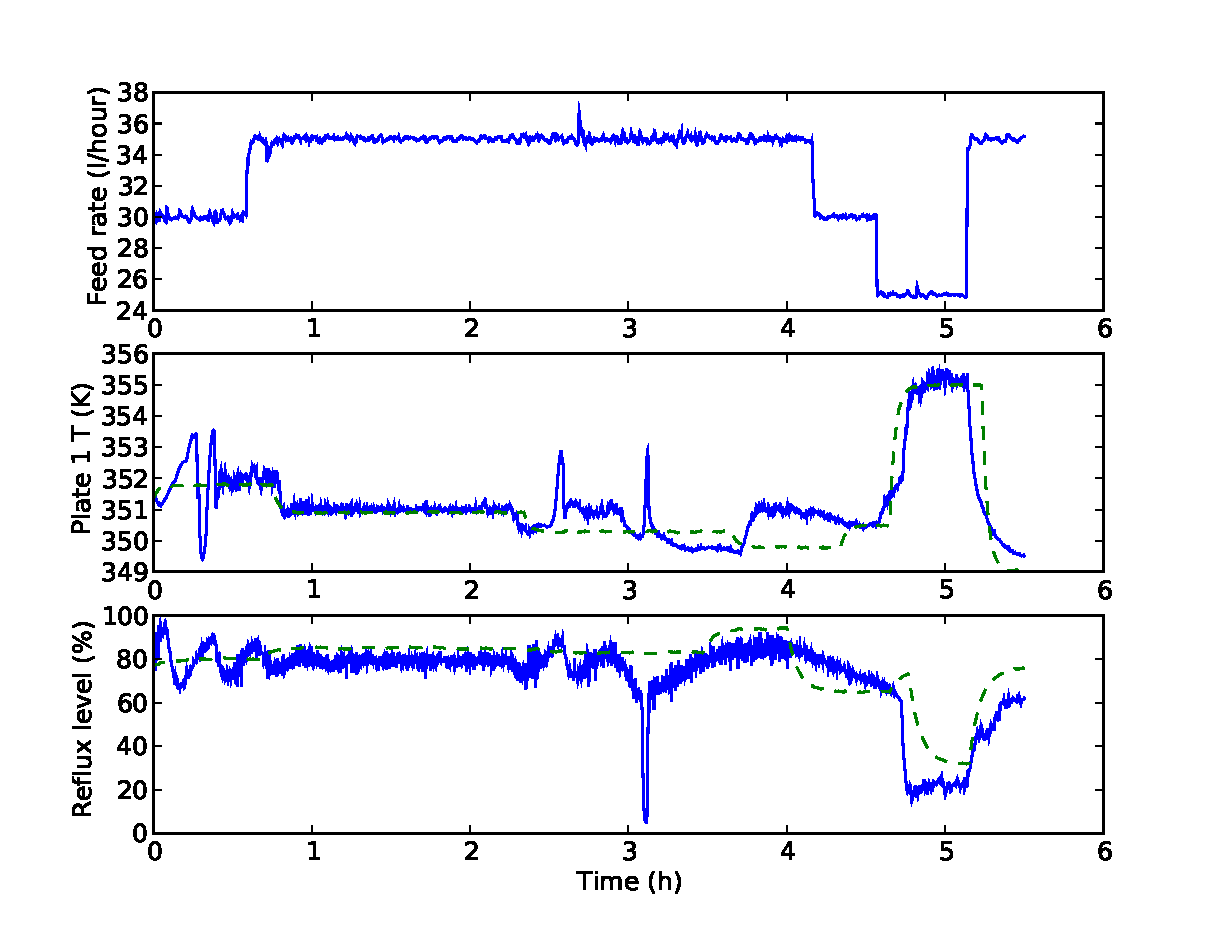
\includegraphics[width=0.9\textwidth]{comparison}
  \caption{Results of simulation compared to measurements. Solid lines are experimental results, dashed lines are model results.}
  \label{fig:comparison}
\end{figure}

It should be noted that the model does not accurately reflect the variation in the reflux drum, probably due to a mismatch between the controller parameters in the model and on the column.  
Further investigation into fitting model parameters should be done.  
However, the overall trends are similar, which is sufficient for this work.

\subsection{Performance profiling}
Real-time operation of the column model proved difficult, and in order to speed up the simulation, profiling of the components making up the simulation was done.  
It was found that the simulation itself could achieve several times real time when simple equilibrium from tables and constant material properties were used instead of the external thermodynamic package.  
As an example, simulating the run shown in Figure~\ref{fig:comparison} takes 30 minutes with simple thermodynamics and 4 hours using the external interface.  
Both the client and the host computers are Pentium 4 Machines with 1GiB of ram.

The high sampling rate of the data (which is sampled at 1 second intervals) may force the integration engine to generate a time point each second, accounting for some of the computational effort. 
However, due to the large difference in running the simulation with and without the external interface, it was surmised that the integration routines of OpenModelica (which uses the DASSL routine from netlib) are not entirely to blame.

In order to better understand the problem, the time spent in handling the network requests was logged.  
This is all the time spent blocked on the network request.  
The results are shown in Figure~\ref{fig:overhead}.
\begin{figure}[htbp]
  \centering
  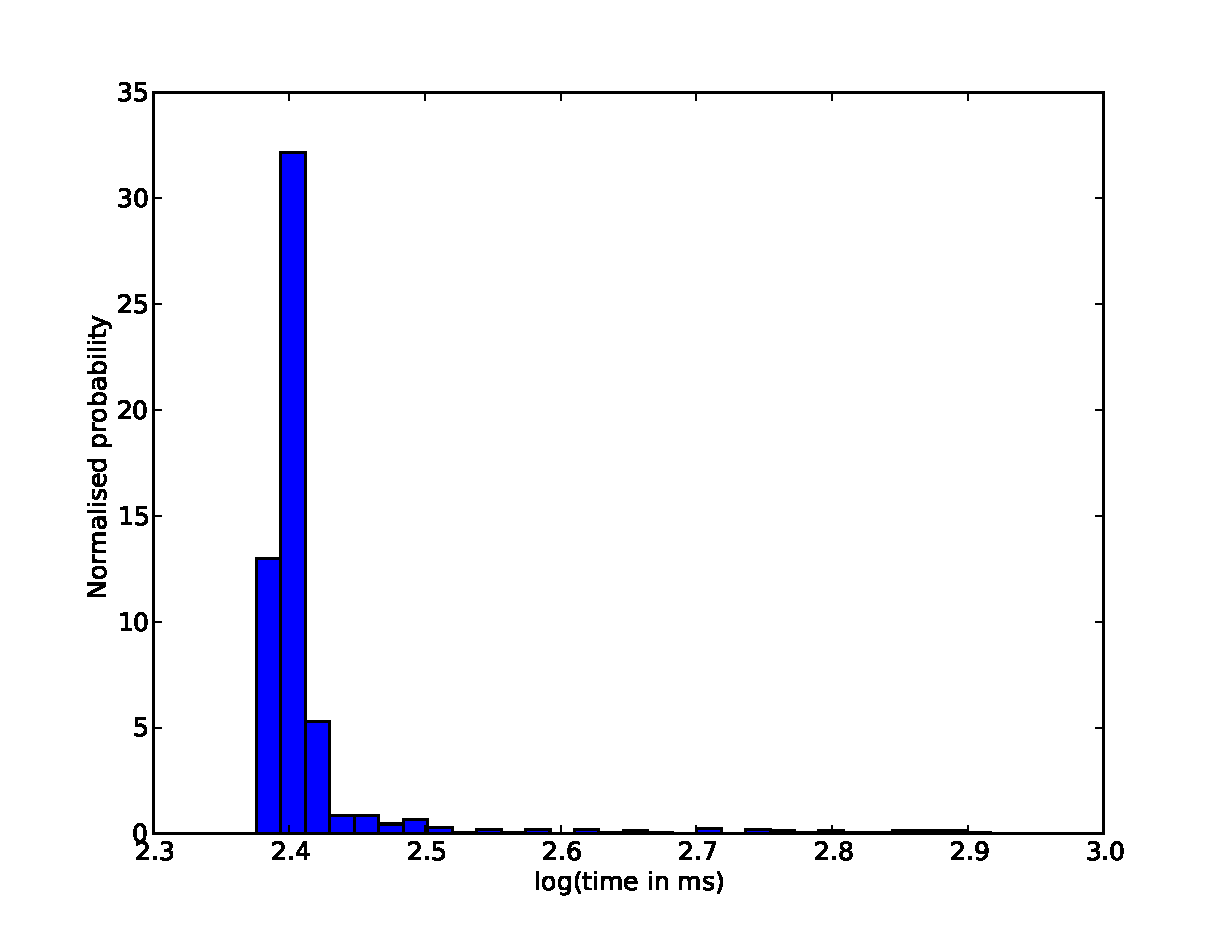
\includegraphics[width=0.6\textwidth]{nethist}
  \caption{Networking overhead for intensive simulation}
  \label{fig:overhead}
\end{figure}
Taking into account that a 30 minute simulation of about 20000 time steps translates to 90 ms per time step and 4 hours 720 ms per time step, it can be seen that the network-blocked part takes about 40\% of the simulation time in most cases, but can take the entire allocated time in some cases.  

The network overhead is therefore significant, even though not all of the performance issues can be attributed solely to the network layer. 
One other possibility that is being pursued is that the compilation of the model files when external routines are being used is not optimal.

A possible explanation for this is that there are SimulationStream instances which all communicate with the server.  
This adds a large overhead due to multiple connections being maintained and property traffic being transmitted simultaneously.  
Currently, work is underway to develop a data broker that will structure the requests to the ORB in a more efficient way.  
The possibility of caching some of the data is also being investigated.

Another explanation is that the external module does not supply derivative information when it is being evaluated, forcing the integration routines to resort to finite differences when estimating the derivatives of these units while solving the equations.  
Attempts are also being made to enable derivative information to be handled by the interface.

\section{Tennessee Eastman Problem}


% Local Variables:
% TeX-master: "thesis"
% End:
